%%%%%%%%%%%%%%%%%%%% book.tex %%%%%%%%%%%%%%%%%%%%%%%%%%%%%
%
% sample root file for the chapters of your "monograph"
%
% Use this file as a template for your own input.
%
%%%%%%%%%%%%%%%% Springer-Verlag %%%%%%%%%%%%%%%%%%%%%%%%%%


% RECOMMENDED %%%%%%%%%%%%%%%%%%%%%%%%%%%%%%%%%%%%%%%%%%%%%%%%%%%
\documentclass[pdftex,12pt, oneside]{book}
 
% choose options for [] as required from the list
% in the Reference Guide, Sect. 2.2
%\usepackage[paperwidth=8.5in, paperheight=13in]{geometry} %Folio
\usepackage[paperwidth=8.27in, paperheight=11.69in]{geometry} %A4

\usepackage{makeidx}         % allows index generation
\usepackage{graphicx}        % standard LaTeX graphics tool
                             % when including figure files
\usepackage[bottom]{footmisc}% places footnotes at page bottom
\usepackage[bahasa]{babel}
\usepackage{enumerate}
\usepackage{paralist}
\usepackage{float}
\usepackage{gensymb}  
\usepackage{listings}
\usepackage{color}
\renewcommand{\baselinestretch}{1.5}

\newcommand{\HRule}{\rule{\linewidth}{0.5mm}}

\makeindex             % used for the subject index
                       % please use the style svind.ist with
                       % your makeindex 
                     
\definecolor{codegreen}{rgb}{0,0.6,0}
\definecolor{codegray}{rgb}{0.5,0.5,0.5}
\definecolor{codepurple}{rgb}{0.58,0,0.82}
\definecolor{backcolor}{rgb}{0.95,0.95,0.92}

\lstdefinestyle{mystyle}{
  backgroundcolor=\color{backcolor},
  commentstyle=\color{codegreen},
  keywordstyle=\color{magenta},
  stringstyle=\color{codepurple},
  basicstyle=\footnotesize,
  breakatwhitespace=false,
  breaklines=true,
  captionpos=b,
  keepspaces=true,
  numbers=left,
  numbersep=5pt,
  showspaces=false,
  showstringspaces=false,
  showtabs=false,
  tabsize=2
}

\lstset{style=mystyle}


%%%%%%%%%%%%%%%%%%%%%%%%%%%%%%%%%%%%%%%%%%%%%%%%%%%%%%%%%%%%%%%%%%%%%

\begin{document}
\sloppy


\begin{titlepage}

\begin{center}
{\large DOKUMENTASI RANCANGAN SISTEM BASIS DATA UNTUK SISTEM INFORMASI PEMBAYARAN PAJAK BUMI DAN BANGUNAN PERDESAAN DAN PERKOTAAN DI KABUPATEN BREBES}

\HRule\\[1cm]

PERIODE PENILAIAN TAHUN 2018\\[1cm]


\includegraphics[width=0.5\textwidth]{./resources/logo}\\[1cm]

Oleh :\\
Priyanto Tamami, S.Kom.\\
NIP 19840409 201001 1 025\\


\vfill


Fungsional Pranata Komputer\\
Badan Pengelolaan Pendapatan, Keuangan dan Aset Daerah\\
Pemerintah Daerah Kabupaten Brebes\\
Brebes, 19 Maret 2018
\end{center}

\end{titlepage}

\frontmatter%%%%%%%%%%%%%%%%%%%%%%%%%%%%%%%%%%%%%%%%%%%%%%%%%%%%%%


\begin{center}
{\huge \bfseries Lembar Pengesahan}\\[0.4cm]

\begin{tabular}{l c p{10cm}}
  Nama Kegiatan & : & 	Membuat Petunjuk Operasional Sistem Komputer \\
  Judul & : & PETUNJUK PENGOPERASIAN PROGRAM SISTEM INFORMASI PEMBAYARAN PAJAK BUMI DAN BANGUNAN PERDESAAN DAN PERKOTAAN DI KABUPATEN BREBES \\
\end{tabular}\\[2cm]

\begin{tabular}{c c}
  Disetujui oleh : & Disusun Oleh \\
  Kepala Sub Bidang Keberatan & Pranata Komputer \\
  Pada tanggal 18 April 2018 & Selesai tanggal : 17 April 2018 \\
  & \\
  & \\
  & \\
  M.L. Setiyawan, S.E.Ak & Priyanto Tamami, S.Kom \\
  NIP 19790530 200604 1 006 & NIP 19840409 201001 1 025
\end{tabular}

\end{center}  

\tableofcontents
\listoffigures

\mainmatter%%%%%%%%%%%%%%%%%%%%%%%%%%%%%%%%%%%%%%%%%%%%%%%%%%%%%%%
\chapter{PENGANTAR}

Untuk membangun sistem ini akan menggunakan bahasa pemrograman Java dengan \textit{framework} Springboot sebagai \textit{service} atau peladen pada bagian belakang (\textit{backend}). Sedangkan pada bagian depan (\textit{frontend}) menggunakan Angular.

Karena basis pemrograman dari Java menggunakan orientasi objek, maka kurang tepat apabila digambarkan dalam diagram \textit{flowchart} yang alur datanya dari atas ke bawah, karena karakteristik pemrograman berorientasi objek alur datanya akan berpindah pindah antar kelas dan \textit{method}.

Ilustrasi yang tepat untuk menggambarkan logika aplikasi dari sistem yang akan dibangun adalah menggunakan UML (\textit{Unified Modelling Language}), dimana diagram akan dipecah kedalam beberapa skenario atau \textit{case} yang telah dibentuk pada saat pengambilan \textit{requirement}.
\chapter{DIAGRAM UNIFIED MODELING LANGUAGE (UML)}

\section{Diagram \textit{Use-Case}}

Diagram \textit{Use-Case} ini akan menjelaskan gambaran menyeluruh atau gambaran besar aktifitas antara pengguna dengan sistem yang dibangun. Diagram \textit{Use-Case} pada sistem informasi ini seperti terlihat pada gambar \ref{fig:use-case} berikut ini :

\begin{figure}[H]
	\centering
	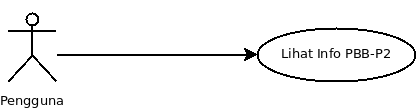
\includegraphics[width=0.5\textwidth]{./resources/uml/use-case-diag}
	\caption{Diagram \textit{Use-Case} Sistem Informasi Pembayaran PBB-P2}
	\label{fig:use-case}
\end{figure}

Yang menjadi aktor disini adalah masyarakat wajib pajak yang melakukan akses ke sistem informasi pembayaran Pajak Bumi dan Bangunan Perdesaan dan Perkotaan (PBB-P2).

\section{Diagram \textit{Class}}

Diagram \textit{class} ini akan menggambarkan hubungan dari tiap kelas yang membangun sistem informasi ini menjadi utuh. Diagram ini akan dibagi menjadi 2 (dua) yang menggambarkan masing-masing bagian antara ujung-depan (\textit{frontend}) dan ujung-belakang (\textit{backend}).

Diagram \textit{class} yang terdapat pada ujung depan (\textit{frontend}) ini seperti pada gambar \textit{fig:class-dia-fe} berikut ini :

\begin{figure}[H]
	\centering
	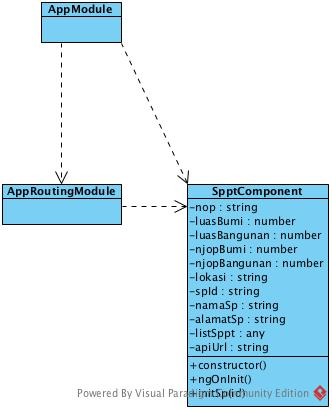
\includegraphics[width=0.5\textwidth]{./resources/uml/class-diagram-fe}
	\caption{Diagram \textit{Class} Untuk Bagian Ujung-Depan (\textit{frontend})}
	\label{fig:class-dia-fe}
\end{figure}

Pada bagian ujung depan (\textit{frontend}), aplikasi akan berakar pada kelas \texttt{AppModule}, kelas \texttt{AppRoutingModule} yang akan mengatur bagaimana tiap komponen kelas (dalam hal ini halaman) akan berganti-ganti sesuai dengan kejadian yang diinginkan oleh pengguna.

Kelas \texttt{AppComponent} dan \texttt{SpptComponent} adalah 2 (dua) kelas yang berhubungan langsung dengan tampilan aplikasi (\textit{view}), keduanya akan dikontrol langsung oleh kelas \texttt{AppRoutingModule} bilamana halaman yang ditampilkan terlebih dahulu apakah \texttt{AppComponent} atau \texttt{SpptComponent}.

Kelas \texttt{AppComponent} sebetulnya kelas yang bertugas menjadi tampilan utama aplikasi, artinya begitu ada \textit{browser} / peramban yang melakukan akses, halaman dari kelas \texttt{AppComponent} ini akan tampil terlebih dahulu menyambut pengguna.

Kelas \texttt{SpptComponent} nanti akan menampilkan informasi yang diminta oleh pengguna berdasarkan Nomor Objek Pajak yang telah dikirimkan melalui formulir atau komponen yang tersedia.

Diagram \textit{class} untuk bagian ujung belakang (\textit{backend}) adalah seperti pada gambar \ref{fig:class-dia-be-1} dan \ref{fig:class-dia-be-2} berikut ini :

\begin{figure}[H]
	\centering
	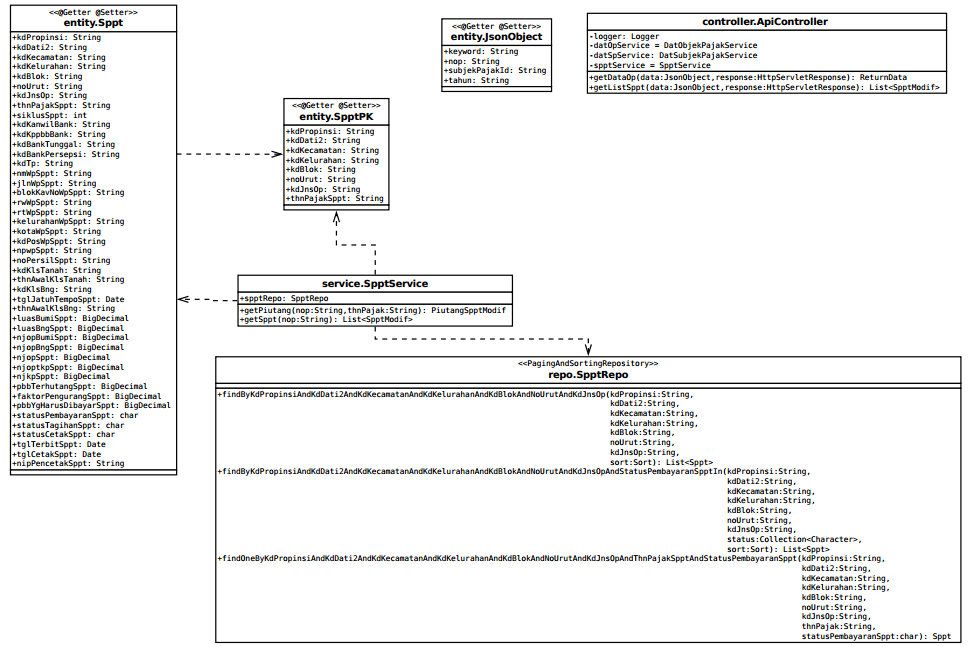
\includegraphics[width=1\textwidth]{./resources/uml/class-dia-be1}
	\caption{Diagram \textit{Class} Untuk Ujung Belakang (\textit{backend}) Bagian 1}
	\label{fig:class-dia-be-1}
\end{figure}

\begin{figure}[H]
	\centering
	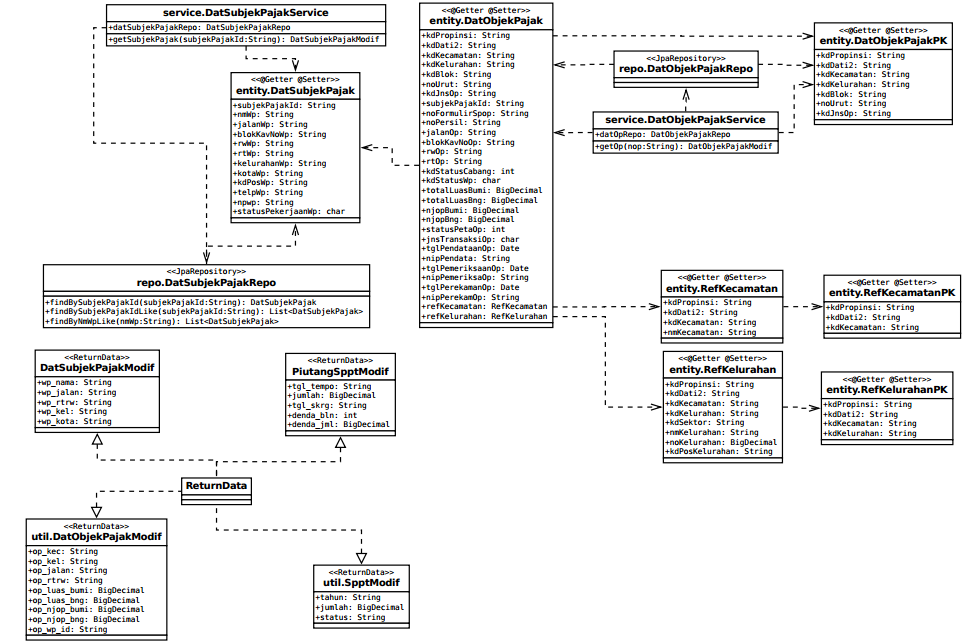
\includegraphics[width=1\textwidth]{./resources/uml/class-dia-be2}
	\caption{Diagram \textit{Class} Untuk Ujung Belakang (\textit{backend}) Bagian 2}
	\label{fig:class-dia-be-2}
\end{figure}

Pada diagram \textit{class} yang pertama, ada kelompok kelas dengan nama yang mirip yaitu \texttt{Sppt}, karena implementasinya menggunakan Spring Data JPA, maka membutuhkan beberapa kelas atau \textit{interface} untuk mengelola data yang berasal dari sistem basis data.

Kelas dan \textit{interface} yang berhubungan dengan tabel \texttt{SPPT} ini adalah seperti berikut :

\begin{itemize}
	\item Kelas \texttt{Sppt}, digunakan untuk melakukan pemetaan atribut pada tabel \texttt{SPPT} pada sistem basis data, isi atributnya akan mirip dengan isi atribut pada tabelnya.
	\item Kelas \texttt{SpptPK}, digunakan untuk mendeklarasikan \textit{primary key} atau kunci utama dari tabel \texttt{SPPT}, nantinya kelas ini akan digunakan pada kelas \texttt{Sppt} untuk memetakan \textit{field-field} yang menjadi \textit{primary key}.
	\item \textit{Interface} \texttt{SpptRepo} adalah deklarasi yang fungsinya untuk melakukan operasi terhadap tabel \texttt{SPPT} di sistem basis data melalui kelas entitas yang berkaitan, dalam hal ini adalah kelas \texttt{SPPT}.
	\item Kelas \texttt{SpptService} digunakan untuk mengelola data atau manipulasi data yang datang dari sistem basis data atau yang akan disimpan ke dalam basis data.
\end{itemize}

Pada diagram \textit{class} bagian pertama ini pun ada 2 (dua) kelas yang tidak berhubungan langsung dengan kelas \texttt{Sppt} yaitu kelas \texttt{JsonObject} yang sebetulnya digunakan untuk pemetaan dari objek JSON yang dikirimkan oleh klien, diubah atau dikonversi menjadi objek Java secara otomatis dengan menggunakan pustaka Jackson. Kemudian kelas yang lain adalah \texttt{ApiController} yang isinya adalah pemetaan URL yang dapat di\textit{request} oleh klien untuk memperoleh data, segala proses yang berhubungan dengan \textit{request} data akan dilakukan pada kelas ini.

Pada diagram \textit{class} bagian kedua akan berisi beberapa kelas dan \textit{interface} yang berhubungan dengan tabel \texttt{DAT\_OBJEK\_PAJAK} beserta beberapa tabel yang berhubungan dengan tabel tersebut.

Adapun kelas-kelas dan \textit{interface} yang ada pada diagram \textit{class} ini yang berhubungan dengan tabel \texttt{DAT\_OBJEK\_PAJAK}, yaitu :

\begin{itemize}
	\item Kelas \texttt{DatSubjekPajakService}, kelas ini bertugas untuk melakukan manipulasi atau pengolahan data yang berasal dari sistem basis data, atau akan disimpan ke sistem basis data.
	\item Kelas \texttt{DatSubjekPajak}, kelas ini berfungsi sebagai kelas pemetaan untuk tabel \texttt{DAT\_SUBJEK\_PAJAK}, maka dari itu isi properti dari kelas ini akan mirip seperti isi properti dari tabel \texttt{DAT\_SUBJEK\_PAJAK}.
	\item \textit{Interface} \texttt{DatSubjekPajakRepo}, \textit{interface} ini berfungsi untuk melakukan operasi terhadap isi data pada tabel \texttt{DAT\_SUBJEK\_PAJAK} seperti simpan data, ubah data, hapus data, ambil data.
	\item Kelas \texttt{DatObjekPajak}, kelas ini berfungsi untuk melakukan pemetaan terhadap tabel \texttt{DAT\_OBJEK\_PAJAK}, seperti kelas \texttt{DatSubjekPajak}, pada kelas ini pun isi propertinya akan mirip seperti pada tabel \texttt{DAT\_OBJEK\_PAJAK}.
	\item \textit{Interface} \texttt{DatObjekPajakRepo}, seperti \textit{interface repository} lainnya, bertugas untuk melakukan manipulasi data pada tabel \texttt{DAT\_OBJEK\_PAJAK} pada sistem basis data.
	\item Kelas \texttt{DatObjekPajakPK}, kelas ini digunakan untuk memetakan \textit{primary key} dari tabel \texttt{DAT\_OBJEK\_PAJAK} yang digunakan oleh kelas \texttt{DatObjekPajak}.
	\item Kelas \texttt{DatObjekPajakService}, kelas ini digunakan untuk mengadaptasikan atau mengolah data dari sistem basis data ke antar muka pengguna, atau sebaliknya, dari antar muka pengguna ke sistem basis data.
	\item Kelas \texttt{RefKecamatan}, kelas ini akan dirujuk oleh kelas \texttt{DatObjekPajak} untuk menampilkan nama wilayah Kecamatan dimana objek berada.
	\item Kelas \texttt{RefKecamatanPK}, kelas ini digunakan sebagai kelas pemetaan untuk \textit{primary key} dari tabel \texttt{RefKecamatan}.
	\item Kelas \texttt{RefKelurahan}, kelas ini digunakan untuk memetakan tabel \texttt{REF\_KELURAHAN} yang digunakan untuk mereferensikan nama wilayah Kelurahan untuk objek pajak terpilih.
	\item Kelas \texttt{RefKelurahanPK}, digunakan untuk memetakan \textit{primary key} dari tabel \texttt{REF\_KELURAHAN} yang akan digunakan pada kelas \texttt{RefKelurahan}.
\end{itemize}

Kelas dan \textit{interface} lain akan berhubungan dengan respon data atau format pemberian data ke klien. Kelas dan \textit{interface} tersebut adalah seperti berikut ini :

\begin{itemize}
	\item \textit{Interface} \texttt{ReturnData}, \textit{interface} ini tidak memiliki isi apapun, hanya untuk menyeragamkan deklarasi kelas-kelas untuk respon data ke klien.
	\item Kelas \texttt{DatSubjekPajakModif}, kelas ini akan mengembalikan nilai-nilai atau informasi mengenai data subjek pajak dari basis data berdasarkan Nomor Objek Pajak (NOP) yang telah diberikan, hanya beberapa informasi saja yang diikutsertakan dalam blok informasi ini sesuai dengan nama propertinya. 
	\item Kelas \texttt{PiutangSpptModif}, kelas ini membawa informasi mengenai data piutang pembayaran pajak bumi dan bangunan sektor perdesaan dan perkotaan (PBB-P2) sesuai dengan Nomor Objek Pajak (NOP) yang diberikan.
	\item Kelas \texttt{DatObjekPajakModif}, kelas ini akan membawa informasi mengenai data informasi objek pajak secara umum seperti tertuang pada propertinya. Tentu saja nilai yang dibawa berdasarkan Nomor Objek Pajak (NOP) yang diberikan.
	\item Kelas \texttt{SpptModif}, kelas ini akan membawa informasi status tagihan pajak berdasarkan tahun pajaknya.
\end{itemize}

Demikianlah isi seluruh kelas dan \textit{interface} yang akan membangun aplikasi pada bagian ujung-belakang (\textit{backend}) agar berjalan sebagaimana mestinya.

\section{Diagram \textit{Component}}

Diagram ini memberikan gambaran hubungan antar komponen, komponen mana yang membutuhkan data dan komponen mana yang memberikan data akan terlihat jelas pada diagram komponen ini.

Diagram \textit{component} untuk bagian ujung-depan (\textit{frontend}) ditunjukkan seperti pada gambar \ref{fig:comp-dia-fe} berikut ini :

\begin{figure}[H]
	\centering
	
\includegraphics[width=1\textwidth]{./resources/uml/component-diagram-fe}
	\caption{Diagram \textit{Component} Untuk Ujung-Depan (\textit{frontend})}
	\label{fig:comp-dia-fe}
\end{figure}

Pada \texttt{AppComponent} sudah terdapat formulir untuk memasukkan Nomor Objek Pajak (NOP), yang apabila diproses maka \texttt{SpptComponent} akan melakukan \textit{request} data ke peladen \textit{Application Programmable Interface} (API) untuk memperoleh data berdasarkan Nomor Objek Pajak (NOP) yang telah dimasukkan oleh pengguna, hasil dari \textit{request} ini akan ditampilkan pada \texttt{SpptComponent} pula.

Diagram \textit{component} yang membentuk bagian ujung belakang (\textit{backend}) adalah seperti pada gambar \ref{fig:comp-dia-be-1}, \ref{fig:comp-dia-be-2}, dan \ref{fig:comp-dia-be-3} berikut ini :

\begin{figure}[H]
	\centering
	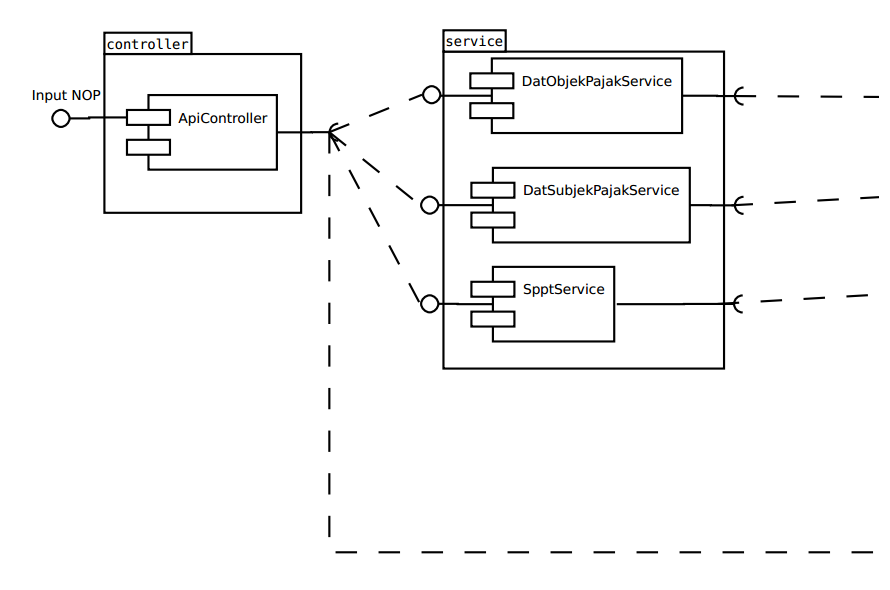
\includegraphics[width=0.7\textwidth]{./resources/uml/comp-dia-backend-1}
	\caption{Diagram \textit{Component} Bagian 1}
	\label{fig:comp-dia-be-1}
\end{figure}

\begin{figure}[H]
	\centering
	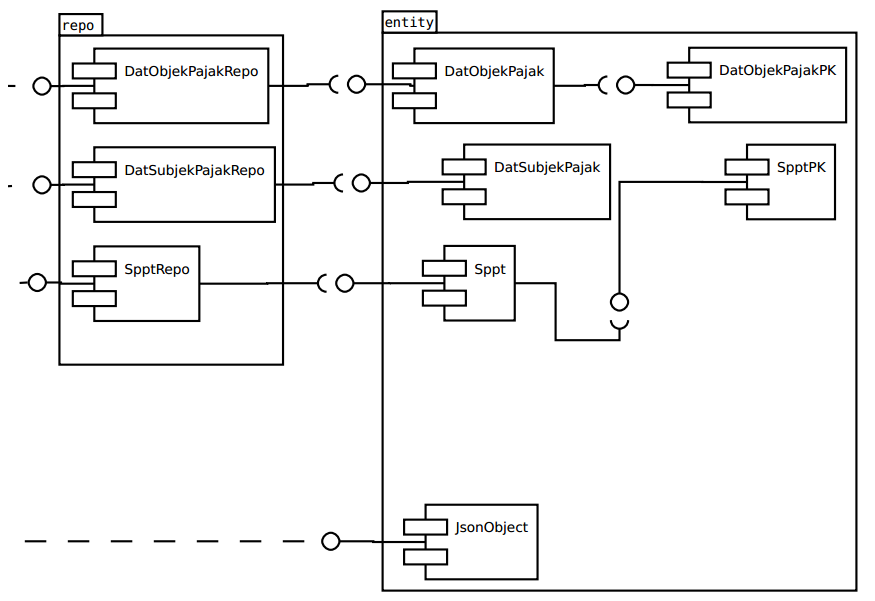
\includegraphics[width=0.7\textwidth]{./resources/uml/comp-dia-backend-2}
	\caption{Diagram \textit{Component} Bagian 2}
	\label{fig:comp-dia-be-2}
\end{figure}

\begin{figure}[H]
	\centering
	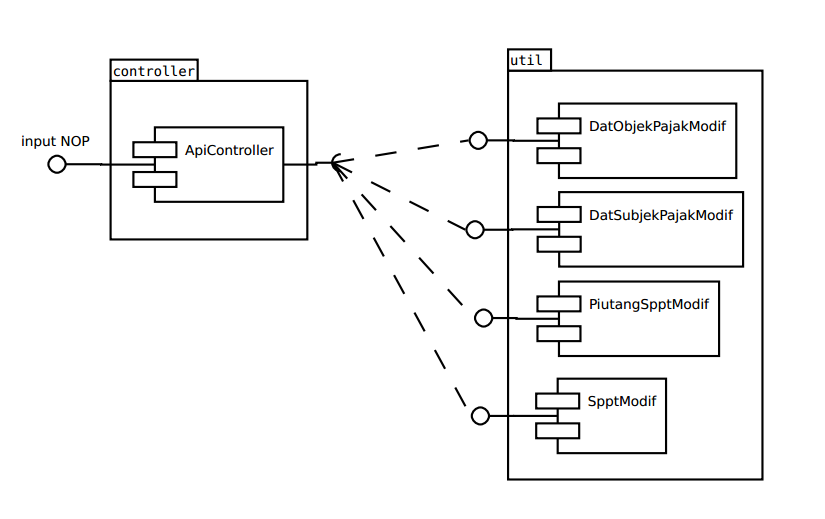
\includegraphics[width=0.7\textwidth]{./resources/uml/comp-dia-backend-3}
	\caption{Diagram \textit{Component} Bagian 3}
	\label{fig:comp-dia-be-3}
\end{figure}

Diagram tersebut berisi komponen yang membangun sistem ini menjadi utuh, begitu ada masukkan data yang terjadi terhadap \texttt{ApiController}, maka \texttt{ApiController} akan menghubungi salah satu atau keseluruhan \textit{service} sesuai dengan \textit{request} yang diterima. Data yang diterima oleh \texttt{ApiController} sebetulnya akan berbentuk JSON, namun akan diterjemahkan otomatis oleh pustaka Jackson ke dalam kelas \texttt{JsonObject} seperti terlihat pada gambar \ref{fig:comp-dia-be-2}.

Kemudian tiap \textit{service} akan melakukan pemanggilan data terhadap \textit{repository}nya masing-masing yang kemudian akan dikembalikan dalam bentuk objek sesuai tabel yang diaksesnya seperti pada gambar \ref{fig:comp-dia-be-1} dan \ref{fig:comp-dia-be-2}.

Hasil yang dikembalikan adalah beberapa objek dari kelas pada paket \texttt{util} seperti disebutkan pada gambar \ref{fig:comp-dia-be-3}

\section{Diagram \textit{Communiation}}

Diagram ini menggambarkan interaksi antar objek yang disertai urutan komunikasi dalam bentuk bagan yang bebas.

Untuk bagian ujung-depan (\textit{frontend}), diagram \textit{communication} diperlihatkan seperti pada gambar ref{fig:comm-dia-fe} berikut ini :

\begin{figure}[H]
	\centering
	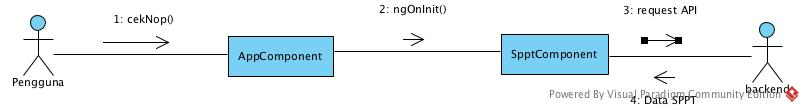
\includegraphics[width=1\textwidth]{./resources/uml/comm-dia-fe}
	\caption{Diagram \textit{Communication} Untuk Bagian Ujung-Depan (\textit{frontend})}
	\label{fig:comm-dia-fe}	
\end{figure}

Alurnya adalah dari pengguna akan memasukkan Nomor Objek Pajak (NOP) pada kolom yang disediakan pada \texttt{AppComponent}, kemudian komponen ini akan memanggil fungsi \texttt{cekNop()} dan mengaktifkan \texttt{SpptComponent} yang secara otomatis akan memanggil fungsi \texttt{ngOnInit()}.

Selanjutnya bagian ujung-depan (\textit{frontend}) akan melakukan \textit{request} ke ujung-belakang (\textit{backend}) yang kemudian ujung belakang akan memberikan data yang diminta dan ditampilkan pada \texttt{SpptComponent}.

Diagram \textit{communication} yang membentuk sistem informasi pajak bumi dan bangunan sektor perdesaan dan perkotaan pada bagian ujung-belakang (\textit{backend}) ini adalah seperti pada gambar \ref{fig:comm-dia-be-1} dan \ref{fig:comm-dia-fe-2} berikut ini :

\begin{figure}[H]
	\centering
	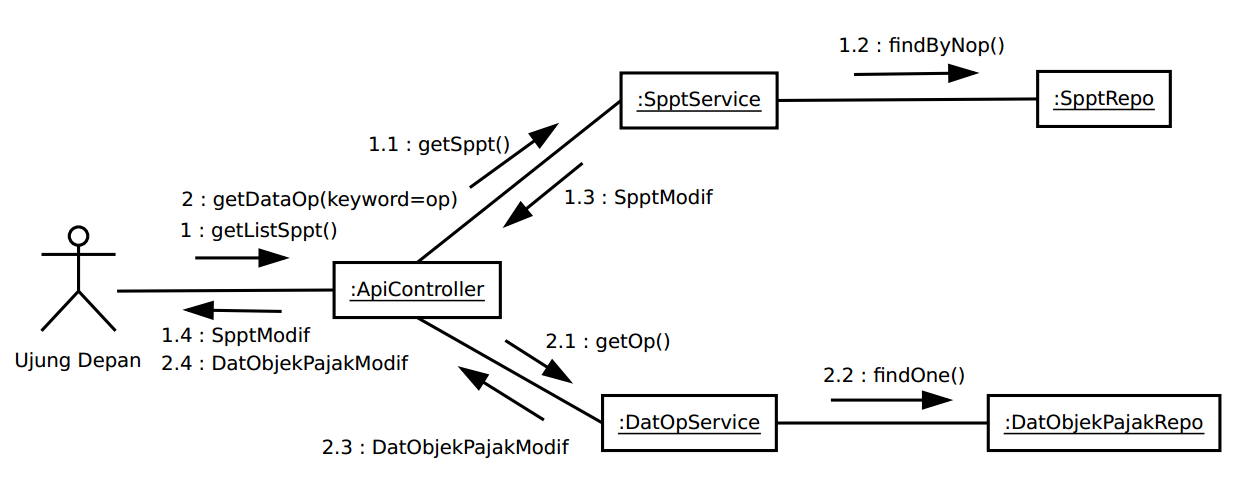
\includegraphics[width=1\textwidth]{./resources/uml/comm-dia-1}
	\caption{Diagram \textit{Communication} Bagian 1}
	\label{fig:comm-dia-be-1}
\end{figure}

\begin{figure}[H]
	\centering
	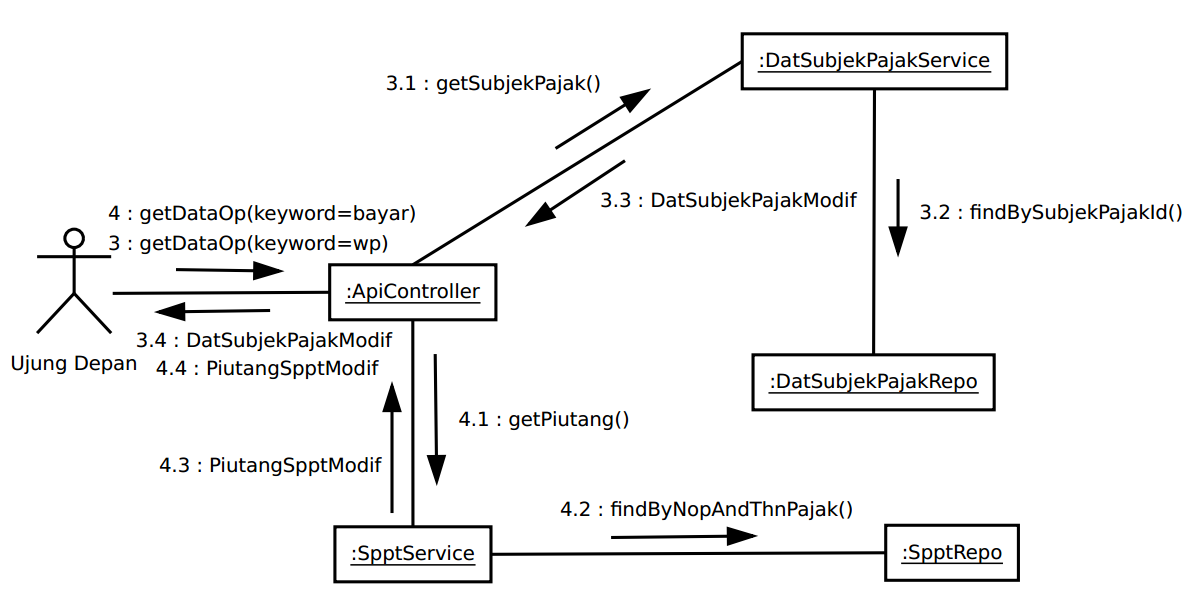
\includegraphics[width=1\textwidth]{./resources/uml/comm-dia-2}
	\caption{Diagram \textit{Communication} Bagian 2}
	\label{fig:comm-dia-be-2}
\end{figure}

Nomor urut 1 (satu) dan 2 (dua) pada saat ujung-depan (\textit{frontend}) berkomunikasi dengan peladen API (dalam hal ini komponen \texttt{ApiController}) bukan berarti urutan dari alur komunikasi melainkan identitas dari skenario. Namun untuk simbol atau angka seperti 1.1 (satu titik satu), 1.2 (satu titik dua), dan seterusnya adalah urutan komunikasi dari skenario 1 (satu) dari langkah pertama sampai langkah ke-n.

Jadi untuk skenario yang ke-1 (satu), bagian ujung-depan (\textit{frontend}) akan memanggil \textit{method} \texttt{getListSppt()} milik kelas \texttt{ApiController}, proses dari skenario ini memanggil \textit{method} \texttt{getSppt()} milik kelas \texttt{SpptService} (pada langkah 1.1), proses selanjutnya akan memanggil \textit{method} \texttt{findByNop()} milik kelas \texttt{SpptRepo} (pada langkah 1.2) yang akhirnya akan mengembalikan ke kelas \texttt{ApiController} dan ke ujung-depan (\textit{frontend}) berupa objek dari kelas \texttt{SpptModif} (pada langkah 1.3 dan 1.4).

Pada skenario ke-2, ujung-depan (\textit{frontend}) akan memanggil \textit{method} \texttt{getDataOp()} milik kelas \texttt{ApiController} dengan parameter \texttt{keyword} berisi teks \texttt{op}, proesnya pertama akan memanggil \textit{method} \texttt{getOp()} milik kelas \texttt{DatOpService} (seperti pada langkah 2.1), kemudian proses berlanjut dengan memanggil fungsi \texttt{findOne()} dari objek kelas \texttt{DatObjekPajakRepo}, hasil dari pemanggilan \textit{method} \texttt{findOne()} ini akan dikonversi ke dalam objek kelas \texttt{DatObjekPajakModif} yang pada akhirnya akan dikembalikan ke aplikasi pada bagian ujung-depan (\textit{frontend}) dalam bentuk JSON.

Pada skenario ke-3 di gambar 4.11, aplikasi bagian ujung-depan (\textit{frontend}) akan melakukan \textit{request} ke \textit{method} \texttt{getDataOp()} dengan parameter \texttt{keyword} berisi teks \texttt{wp}. Langkah selanjutnya adalah memanggil \textit{method} \texttt{getSubjekPajak()} milik kelas \texttt{DatSubjekPajakService}, yang prosesnya kemudian akan memanggil \textit{method} \texttt{findBySubjekPajakId()}, hasilnya kemudian akan disesuaikan masuk ke dalam kelas \texttt{DatSubjekPajakModif} yang dikembalikan ke bagian ujung-depan (\textit{frontend}).

Skenario ke-4 sama saja seperti skenario ke-3 dan ke-2, akan memanggil \textit{method} \texttt{getDataOp()} dengan parameter \textit{keyword} berisi teks \texttt{bayar}. Langkah selanjutnya adalah memanggil \textit{method} \texttt{getPiutang()} milik kelas \texttt{SpptService} yang kemudian akan mengambil data ke sistem basis data dengan memanggil \textit{method} \texttt{findByNopAndThnPajak()} milik kelas \texttt{SpptRepo}. Hasil dari proses ini akan mengembalikan ke bagian ujung-depan (\textit{frontend}) berupa objek dari kelas \texttt{PiutangSpptModif} dalam bentuk JSON.

\section{Diagram \textit{Activity}}

Diagram ini masuk dalam kategori diagram \textit{behavior} yang menunjukkan alur kontrol atau alur objek yang dipertegas dalam urutan aktivitas dan kondisi pada alur yang terjadi.

Diagram \textit{activity} untuk bagian ujung-depan (\textit{frontend}) adalah seperti terlihat pada gambar \ref{fig:act-dia-fe} berikut ini :

\begin{figure}[H]
	\centering
	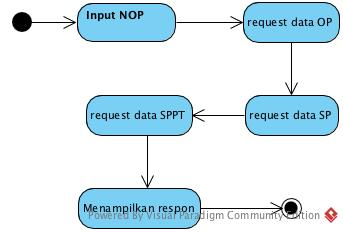
\includegraphics[width=1\textwidth]{./resources/uml/act-dia-fe}
	\caption{Diagram \textit{Activity} Untuk Bagian Ujung-Depan (\textit{frontend})}
	\label{fig:act-dia-fe}
\end{figure}

Terlihat pada diagram tersebut bahwa bagian ujung-depan (\textit{frontend}) akan melakukan 3 (tiga) kali \textit{request} atau permintaan data ke peladen API (\textit{Application Programmable Interface}), kemudian menampilkan hasil yang diberikan oleh peladen ke jendela \textit{browser} / peramban.

Pada bagian ujung-belakang (\textit{backend}), diagram \textit{activity} ini akan terbagi berdasarkan skenario yang telah terbentuk pada Diagram \textit{communication} sebelumnya.

Pada skenario pertama, adalah aktivitas yang terjadi ketika ada \textit{request} daftar tagihan pajak bumi dan bangunan sektor perdesaan dan perkotaan dari klien, diagram \textit{activity} untuk skenario ini adalah seperti pada gambar \ref{fig:act-dia-be-1} berikut ini :

\begin{figure}[H]
	\centering
	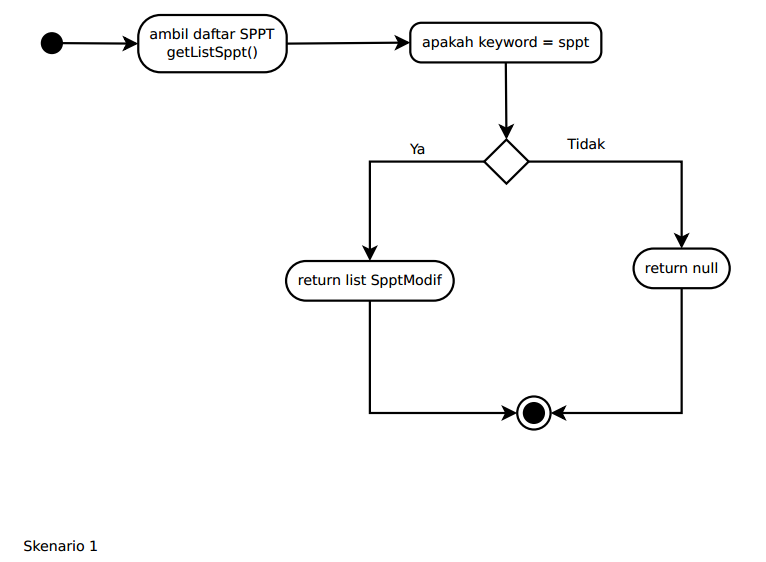
\includegraphics[width=1\textwidth]{./resources/uml/activity-dia-1}
	\caption{Diagram \textit{Activity} Untuk Ambil Daftar Tagihan}
	\label{fig:act-dia-be-1}
\end{figure}

Diagram tersebut menunjukkan apabila data yang diminta oleh klien tidak ada pada sistem basis data, maka sistem akan mengembalikan nilai \texttt{null} atau kosong.

Skenario yang kedua terjadi ketika ada \textit{request} data objek pajak dari klien. Diagram \textit{activity} untuk skenario kedua ini seperti terlihat pada gambar \ref{fig:act-dia-be-2} berikut ini :

\begin{figure}[H]
	\centering
	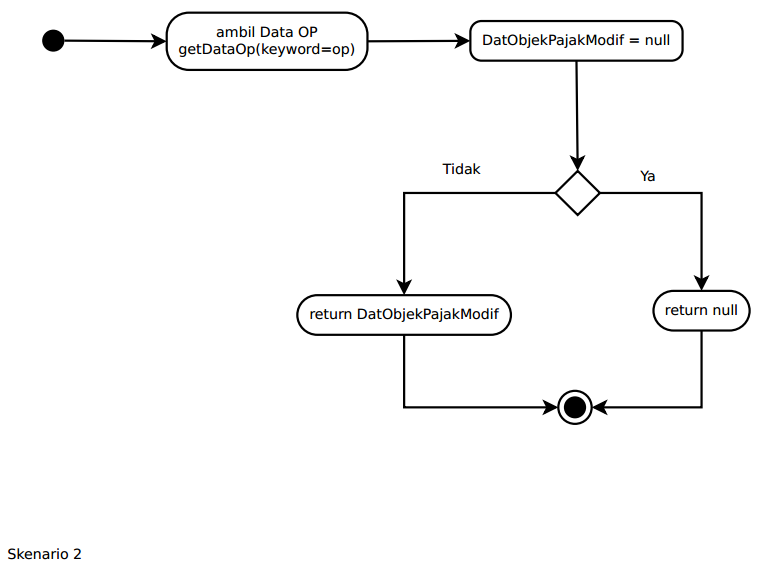
\includegraphics[width=1\textwidth]{./resources/uml/activity-dia-2}
	\caption{Diagram \textit{Activity} Skenario Kedua}
	\label{fig:act-dia-be-2}
\end{figure}

Skenario berikutnya adalah skenario ketiga, yang terjadi ketika ada \textit{request} data wajib pajak dari klien. Diagram \textit{activity} untuk skenario ini adalah seperti pada gambar \ref{fig:act-dia-be-3} berikut ini :

\begin{figure}[H]
	\centering
	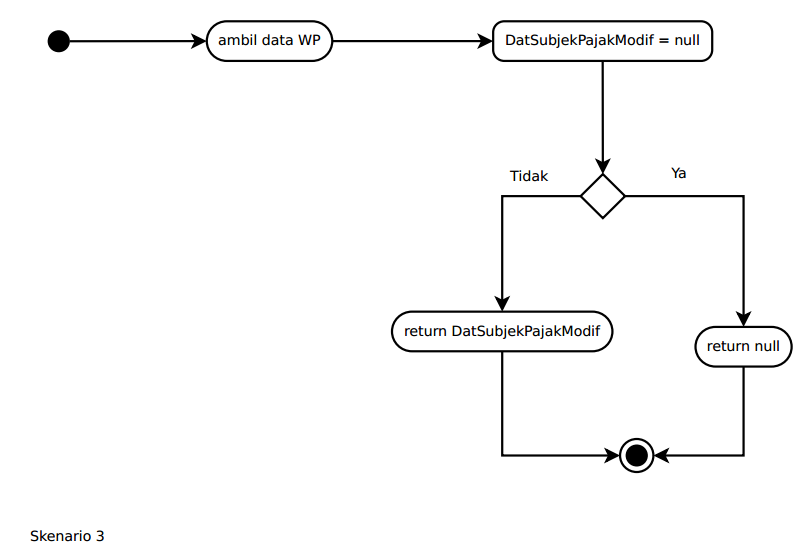
\includegraphics[width=1\textwidth]{./resources/uml/activity-dia-3}
	\caption{Diagram \textit{Activity} Skenario Ketiga}
	\label{fig:act-dia-be-3}
\end{figure}

Skenario keempat terjadi ketika ada \textit{request} data pembayaran dari klien. Diagram \textit{activity} untuk skenario ini adalah seperti pada gambar \ref{fig:act-dia-be-4} berikut ini :

\begin{figure}[H]
	\centering
	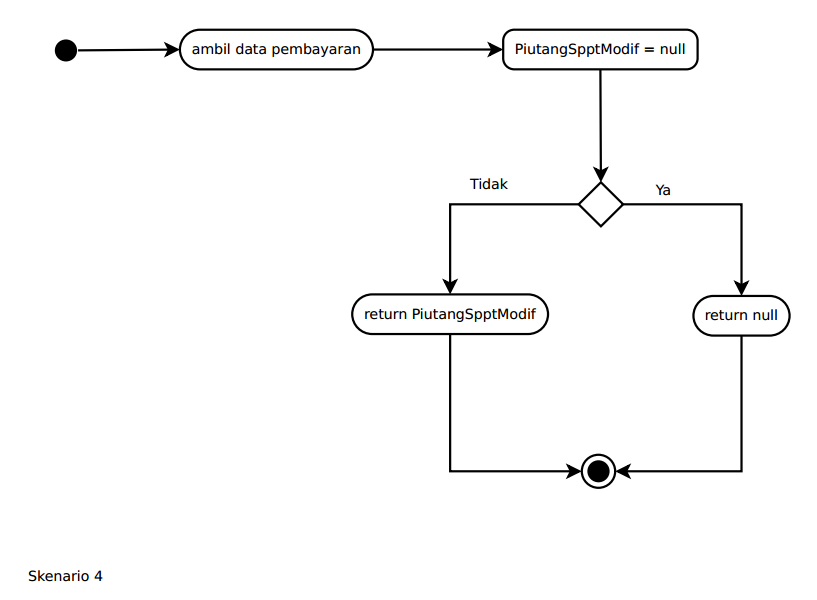
\includegraphics[width=1\textwidth]{./resources/uml/activity-dia-4}
	\caption{Diagram \textit{Activity} Skenario Keempat}
	\label{fig:act-dia-be-4}
\end{figure}

\section{Diagram \textit{Sequence}}

Diagram ini akan menggambarkan alur pertukaran pesan dari beberapa objek pada rentang siklus hidupnya.

Untuk bagian ujung-depan (\textit{frontend}), diagram \textit{sequence} yang menggambarkan alur kontrol adalah seperti pada gambar \ref{fig:seq-dia-fe} berikut ini :

\begin{figure}[H]
	\centering
	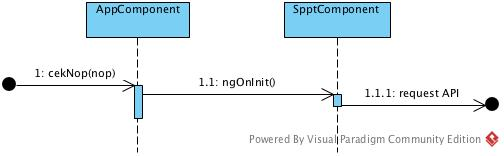
\includegraphics[width=1\textwidth]{./resources/uml/seq-dia-fe}
	\caption{Diagram \textit{Sequence} Untuk Bagian Ujung-Depan (\textit{frontend})}
	\label{fig:seq-dia-fe}
\end{figure}

Prosesnya terlihat cukup sederhana, yaitu dari saat pengguna memasukkan Nomor Objek Pajak pada komponen yang tersedia, kemudian begitu pengguna melakukan klik pada tombol yang disediakan, maka otomatis akan memanggil fungsi \texttt{cekNop()} dengan parameter berupa Nomor Objek Pajak (NOP), kemudian aplikasi akan membuka / memanggil \texttt{SpptComponent} yang di dalamnya kemudian melakukan \textit{request} terhadap API (\textit{Application Programmable Interface}) pada peladen bagian ujung belakang (\textit{backend}). 

Pada bagian ujung-belakang (\textit{backend}), diagram ini pun terbentuk dari skenario-skenario yang terjadi dari diagram \textit{communication} sebelumnya.

Pada skenario pertama, sistem akan memberikan daftar tagihan pajak bumi dan bangunan sektor perdesaan dan perkotaan untuk seluruh wajib pajak berdasarkan Nomor Objek Pajak (NOP) yang diminta.

Diagram \textit{sequence} untuk skenario pertama ini seperti pada gambar \ref{fig:seq-dia-be-1} berikut ini :

\begin{figure}[H]
	\centering
	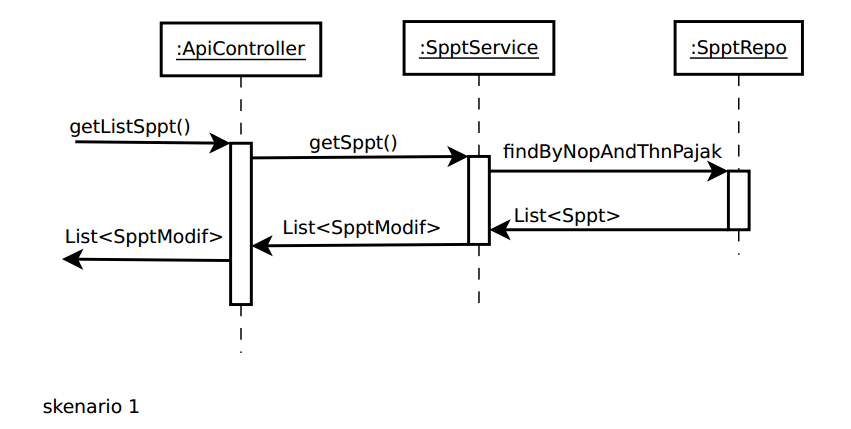
\includegraphics[width=1\textwidth]{./resources/uml/seq-dia-1}
	\caption{Diagram \textit{Sequence} Untuk Skenario Pertama}
	\label{fig:seq-dia-be-1}
\end{figure}

Untuk skenario kedua, sistem akan memberikan informasi mengenai objek pajak berdasarkan Nomor Objek Pajak (NOP) yang diminta. Diagram \textit{sequence} untuk skenario ini adalah seperti pada gambar \ref{fig:seq-dia-be-2} berikut ini :

\begin{figure}[H]
	\centering
	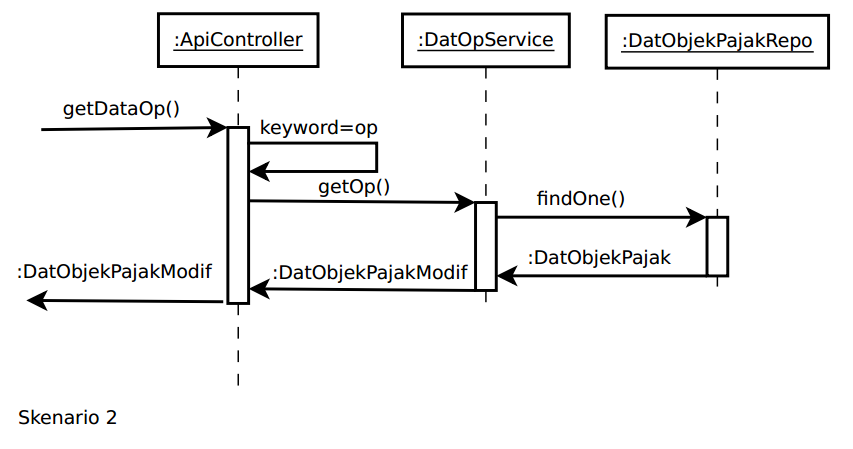
\includegraphics[width=1\textwidth]{./resources/uml/seq-dia-2}
	\caption{Diagram \textit{Sequence} Untuk Skenario Kedua}
	\label{fig:seq-dia-be-2}
\end{figure}

Untuk skenario ketiga, sistem akan memberikan informasi mengenai wajib pajak berdasarkan Nomor Objek Pajak (NOP) yang diminta. Diagram \textit{sequence} untuk skenario ini adalah seperti pada gambar \ref{fig:seq-dia-be-3} berikut ini :

\begin{figure}[H]
	\centering
	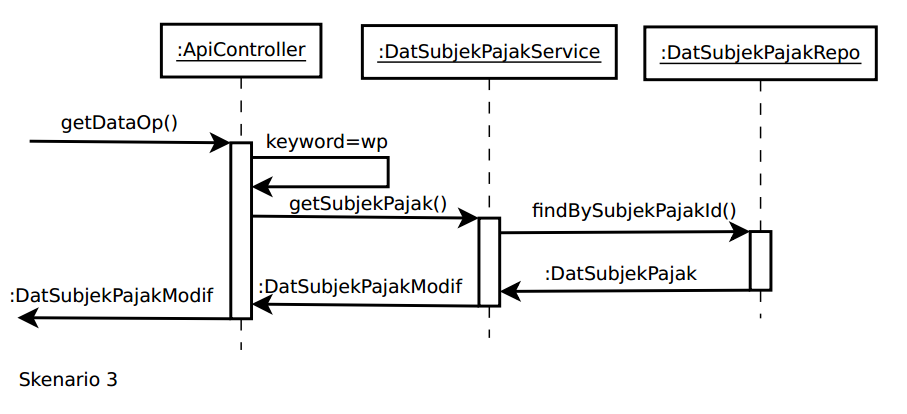
\includegraphics[width=1\textwidth]{./resources/uml/seq-dia-3}
	\caption{Diagram \textit{Sequence} Untuk Skenario Ketiga}
	\label{fig:seq-dia-be-3}
\end{figure}

Untuk skenario keempat, sistem akan memberikan tanggal jatuh tempo dan denda (apabila ada karena keterlambatan pembayaran) untuk objek pajak berdasarkan Nomor Objek Pajak (NOP) dan tahun pajak tertentu. Diagram \textit{sequence} untuk skenario ini adalah seperti pada gambar \ref{fig:seq-dia-be-4} berikut ini :

\begin{figure}[H]	
	\centering
	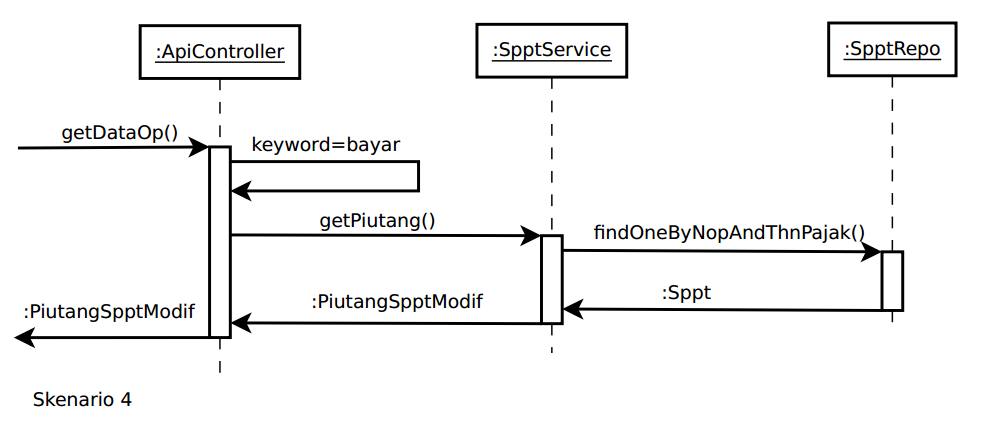
\includegraphics[width=1\textwidth]{./resources/uml/seq-dia-4}
	\caption{Diagram \textit{Sequence} Untuk Skenario Keempat}
	\label{fig:seq-dia-be-4}
\end{figure}

\section{Diagram \textit{Deployment}}

Diagram ini menunjukkan arsitektur dari sistem pada saat didistribusikan dari mesin tempat untuk mengembangkan dan uji coba, ke mesin produksi tempat aplikasi siap melayani pengguna aslinya.

Diagram ini digambarkan seperti pada gambar \ref{fig:deploy-dia} berikut ini :

\begin{figure}[H]
	\centering
	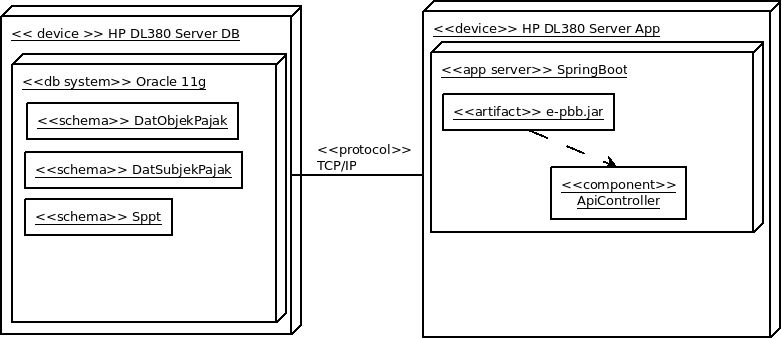
\includegraphics[width=1\textwidth]{./resources/uml/deploy-diagram}
	\caption{Diagram \textit{Deployment}}
	\label{fig:deploy-dia}
\end{figure}

Pada diagram tersebut ditunjukkan bahwa sistem aplikasi ini menggunakan 2 (dua) peladen, yang pertama untuk sistem basis data seperti ditunjukkan pada gambar yang memiliki sistem basis data (perangkat / \textit{device} di sebelah kiri), dan yang kedua adalah peladen sebagai aplikasi dengan Tomcat dan lingkungan berada dalam satu paket pada Springboot.


\backmatter%%%%%%%%%%%%%%%%%%%%%%%%%%%%%%%%%%%%%%%%%%%%%%%%%%%%%%%
\printindex

%%%%%%%%%%%%%%%%%%%%%%%%%%%%%%%%%%%%%%%%%%%%%%%%%%%%%%%%%%%%%%%%%%%%%%

\end{document}





